\chapter[Procedimentos Metodológicos e Técnicas]{Procedimentos Metodologia e Técnicas}

Estarão citadas aqui as formas e técnicas que foram utilizadas para a realização deste trabalho, e quaisquer outras formas metodológicas utilizadas durante o desenvolvimento do mesmo. 

\section{O Processo de Desenvolvimento}

O sistema será desenvolvido baseando-se em uma forma mais simples da metodologia ágil SCRUM. Utilizando uma metodologia ágil de desenvolvimento, o projeto teve pequenas iterações incrementais de uma semana com um valor visível, ou seja, com mudanças aparentes ou novas funcionalidades implementadas. 

Ao final de cada semana, houve uma revisão do trabalho com o que foi realizado e o que ainda precisa ser realizado, aonde foi planejado o que se fazer para a próxima iteração. 

Não houve programação em pares devido a restrições do trabalho e não houve reuniões diárias pelo fato de não haver um \textit{scrum master} associado ao projeto e nem um cliente em si. As revisões semanais das iterações foram realizadas com o orientador do projeto que serviram de uma forma similar a um cliente e \textit{scrum master}, dando opiniões e comentários sobre o andamento do projeto.

\section{A API Gráfica do Sistema}

Devido a facilidade de programação para jogos e prévio conhecimento, a linguagem de programação utilizada para o desenvolvimento da ferramenta utilizada foi escolhida como C++. 

Dentro das API's mais conhecidas para programação de jogos em C++, gratuitas, encontram-se: 
\begin{itemize}
	\item Allegro 5 
	\item SDL 2
	\item SFML 2.1
\end{itemize}

Allegro é uma API conhecida por sua simplicidade, porém devido a prévias tentativas e problemas encontrados em sua versão 4 com placas gráficas \textit{onboard} está não foi realmente considerada como uma opção viável para o momento, dado também o tempo de aprendizado adicional que seria necessário para seu domínio.

A SDL é uma ferramenta que recentemente disponibilizou sua versão 2.0 com grandes mudanças e melhoras de performance, podendo-se dizer com facilidade que é uma das mais conhecidas e utilizadas das três API's (baseado em sua versão 1.0), assim como a mais antiga. É construída C, apesar de garantir suporte nativo a C++.

A SFML é uma API relativamente recente que utiliza-se de diversos benefícios da linguagem C++11 internamente para segurança e integridade. Seus benefícios se dão pela sua construção orientada a objetos, o que facilita na utilização e organização de seus diversos módulos.

Todas as API's descritas são multiplataformas e permitem a compilação de aplicativos para Windows, Linux e MacOS.

Um breve comparativo entre SDL e SFML foi realizado, cujos resultados estão compilados na Tabela 1 (\ref{tab01}).

\begin{table}[h]
	\centering
	\label{tab01}
	
	\begin{tabular}{lll}
		\toprule
		\textbf{Característica} & \textbf{SDL} & 
		\textbf{SFML} \\
		\midrule
		Multiplataforma 			& Sim & Sim \\
		Orientado a Objetos 		& Não & Sim \\
		Aceleração de Hardware   	& Sim & Sim \\
		Integração com Áudio		& Sim, através de bibliotecas & Sim \\
		Integração com imagens \textit{.png} e \textit{.jpg} & Sim, através de bibliotecas & Sim \\
		Alto Grau de Maturidade		& Sim & Não* \\
		Referências e exemplos		& Sim & Não**\\
		\textit{Open Source}					& Sim & Sim\\
		\bottomrule
	\end{tabular}

	\caption{Comparativo entre SDL e SFML}
\end{table}

*A SFML, por ser uma API relativamente mais nova, ainda não possui o mesmo nível de maturidade que o SDL possui vindo de exaustivos testes e utilizações por usuários ao longo dos anos.

**A SFML, por ser mais recente e só agora começar a ser mais divulgada, ainda não possui uma grande base de tutoriais externos além dos presentes no site oficial e o seu manual de API.

Por fim, foi escolhido a utilização da SFML devido a suas facilidades, orientação a objetos nativa e objetos primitivos pré-construidos como classes para representação de textos e gráficos.

Foi também utilizado a biblioteca Qt 5 para o interfaceamento gráfico, principalmente da ferramenta auxiliar. O Qt disponibiliza diversas características comuns para janelas como menus, botões, e outros padrões gráficos que usuários estão acostumados a esperar de ferramentas. A utilização desta biblioteca torna ferramenta o mais intuitiva e efetiva possível, enquanto as API's citadas acima, que são muito bem utilizadas para jogos, falham em ter uma padronização de interface, dando a liberdade ao programador de faze-las, o que para o contexto de um jogo é algo desejável. Por isso foi-se utilizado o SFML para a produção dos gráficos e contextos da simulação e o Qt para a produção da ferramenta.

\section{Simulação}

O primeiro passo para o projeto foi a construção de uma ferramenta confiável que permitisse um ambiente de simulação controlado para os testes que devem ser executados sobre o mapa. E o jogo, apesar de simplificada, deve conter os elementos principais de um rogo \textit{roguelike} para poder-se comparar a efetividade de cada mapa para este gênero.

A simulação do jogo presente na ferramenta principal consta de regras básicas para que se possa testar, da forma mais genérica possível, jogos do gênero \textit{roguelike}. O jogador iniciará em um nível carregado a partir de um arquivo externo ou gerado por um algoritmo procedural lido pela ferramenta. O nível carregado deverá ter, mínimamente, um ponto de entrada e um ponto de saída, podendo também haver uma série de inimigos e itens de diferentes atributos espalhados pelo mapa. 

Para facilitar o entendimento do sistema os itens estarão limitados a itens de recuperação, que aumentarão a quantidade de vida do jogador, e itens de atributos, que aumentarão a quantidade de ataque ou defesa do jogador até o termino do nível, se coletados.

\subsection{Turnos}
A simulação se desenvolve em turnos. Um turno só ocorrerá caso o jogador faça um movimento, que pode ser um movimento a um espaço vazio ao seu redor, ou um ataque a um inimigo adjacente. Ao realizar um turno, todos os outros inimigos do mapa irão também realizar seus turnos e mover-se em direção ao jogador para atacá-lo, caso estejam em sua área de observação. 

A sucessão dos turnos se baseia em um atributo de custo de velocidade. Cada movimento do jogador irá causar no sistema a passagem de $t$ unidades de tempo, sendo este número igual a quantidade de custo que o jogador necessita para realizar um movimento (turno). Inimigos mais comumente possuirão um atributo de custo para se moverem maior que o jogador, tornando assim possível um jogador lutar contra diversos inimigos mais fracos com chances reais de vitória.

Para o caso do jogador se mover e o inimigo não atingir o seu valor de custo para movimentação, este valor é armazenado e utilizado para o próximo turno, decrementando somente a quantidade utilizada ao se mover. Por exemplo: Um jogador com custo de movimento $100$ se move e é visto por um inimigo de custo $150$. O inimigo não se moverá, porém terá $100$ de custo armazenado. O jogador realiza outro passo, deixando-o agora com $200$ armazenado, o qual realiza o seu movimento de custo $150$ e deixa armazenado $50$ para o próximo turno, no qual conseguirá novamente se mover, sobrando zero e repetindo este processo (Figura 7 - \ref{fig07}).
\\\\
\begin{figure}[h]
	\centering
	\label{fig07}
		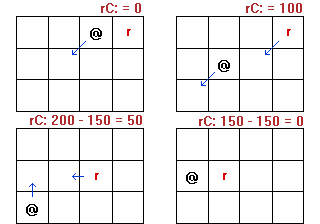
\includegraphics[keepaspectratio=true,scale=0.8]{figuras/fig07-turn.png}
	\caption{Desenvolvimento de Turnos}
\end{figure}

\subsection{Mapas}

O mapa é dividido em \textit{tiles} (blocos). Cada bloco é representado por um quadrado que pode ser passável ou não. Em cada bloco pode haver até um item ou um inimigo ao mesmo tempo. Jogadores ao passarem por cima de itens, irão consumí-los para aumentar seus atributos ou recuperar sua vida. E não poderá haver jogadores e inimigos coexistindo ao mesmo tempo em um bloco, havendo um ataque caso um inimigo ou jogador esteja tentando se mover para um bloco ocupado.

A ferramenta terá a capacidade de leitura de um arquivo externo \textit{.map}, que nada mais é que um arquivo de texto com a devida formatação entendida pelo sistema. O arquivo terá informações sobre a localidade inicial do jogador, os blocos do mapas e possíveis inimigos e itens espalhados por ele.

\subsubsection{Blocos}
Os primeiros valores do arquivo representam a disposição do mapa em relação ao seu tamanho, posição inicial do jogador, tipos e gráficos dos blocos.
A formatação segue o padrão:
\begin{verbatim}
	P_x . P_y
	map_X-map_Y
	id:tipo  id:tipo ...
\end{verbatim}
	
Os primeiros dois valores P\_x e P\_y representam a posição inicial do jogador (a qual deve ser um bloco passável),sendo separados por um ponto.
Na linha seguinte será indicado o tamanho nas direções do mapa em X e Y, com ambos valores separados por um traço.
As map\_Y linhas seguintes, representarão os blocos. Cada linha terá map\_X identificadores dispostos por um $id$ e $tipo$, separados por dois-pontos. 

Cada conjunto de $id:tipo$ representa o bloco na sua posição de acordo com sua linha/coluna.
Um identificador de um bloco pode ser: 

	\begin{itemize}
		\item 0 - Bloco não passável
		\item Maior que 1 - Bloco passável
	\end{itemize}

O segundo identificador $tipo$ é o representativo visual que o bloco terá dentro do jogo. O $tipo$ nada mais é do que um índice de recorte utilizado de um arquivo carregado pela ferramenta encontrado em \textit{"data/img/tileset.png"}. Este arquivo pode ser de qualquer tamanho, e o jogo irá utilizá-lo para extrair o seus blocos. A imagem será recortada em pedaços de 16x16 pixels e será atribuída cada pedaço a um índice. Desta forma um \textit{tileset.png} de 160x32 pixels terá índices entre 0 e 19 para representações. Os índices crescem horizontalmente, e ao chegar ao final de uma linha  vão para a linha de baixo.  

\begin{figure}[h]
	\centering
	\label{fig08}
		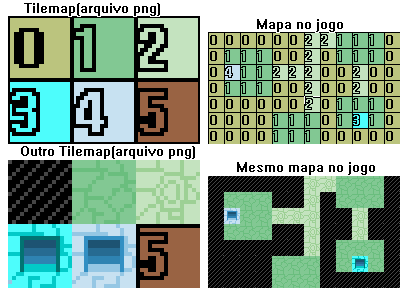
\includegraphics[keepaspectratio=true,scale=0.5]{figuras/fig08-map.png}
	\caption{Mapa, '3' e '4' indicando pontos de saída e entrada do mapa}
\end{figure}

\subsubsection{Inimigos e Itens}

Uma linha imediatamente após o último bloco ser descrito no arquivo \textit{.map}, haverá então os itens e inimigos presentes no mapa.
Ao contrário dos blocos, os inimigos e itens não precisam ser dispostos seqüencialmente de acordo com suas posições e podem estar intercalados entre si.

Existem 3 variações possíveis de entradas nesta parte do formato. Elas são identificadas por uma linha contendo os seguintes textos:
\begin{itemize}
	\item ``\textit{Item}:'' - Itens de recuperação de vida ou de incrementos de atributos.
	\item ``\textit{Gold}:'' - Dinheiro, para simulação dos benefícios do nível.
	\item ``\textit{Enemy}:'' - Inimigos.
\end{itemize}

A linha subseqüente a um destes três textos conterá uma seqüencia de valores representando suas características. Em todos os três casos, os valores iniciam-se por dois identificados: $x$,$y$, representando as coordenadas do bloco $x$, $y$ em que serão colocados.
\subsubsubsection{\textit{Gold} - Dinheiro} 
O mais simples deles, contém apenas mais uma variável $g$ que representa a quantidade de dinheiro. O \textit{sprite} escolhido para o dinheiro é automaticamente
definido pelo sistema. Os primeiros seis \textit{sprites} do mapa de itens representam os estados do dinheiro, que são definido como:
\begin{itemize}
	
	\item 1-5g -    \textit{Sprite} 0
	\item 6-15g -   \textit{Sprite} 1
	\item 16-30g -  \textit{Sprite} 2
	\item 31-50g -  \textit{Sprite} 3
	\item 51-100g - \textit{Sprite} 4
	\item 100g+ -   \textit{Sprite} 5
\end{itemize}

%34,14,6,3,1,4,200,3,0
\subsubsubsection{\textit{Enemy} - Inimigo} 
Descrito pelos atributos: \texttt{hp},\texttt{atk},\texttt{def},\texttt{range},\texttt{cost},\texttt{sprIDx}, \texttt{sprIDy}.
Os primeiros valores são os atributos básicos do inimigo: sua vida, ataque e defesa.

O valor de $range$ indica a visão do inimigo, isto é, a quantidade de blocos de distância que ele conseguirá observar o jogador e tomar a decisão de atacá-lo.
O valor $cost$ representa o custo de movimentação do inimigo, ou seja, quanto menor o valor, mais rápido será o inimigo.
Por fim, os últimos dois valores representam a posição X e Y do arquivo gráfico para visualização do inimigo (\textit{data/img/chars.png}).

\subsubsubsection{Item} 
Este é o mais complicado dentre os três tipos de entrada do mapa, uma vez que pode abranger tipos de itens diferentes em uma mesma linha.
É determinado pelos valores: \texttt{buff}, \texttt{hp}, \texttt{mp}, \texttt{atk}, \texttt{def}, \texttt{sprIDx}, \texttt{sprIDy}

O primeiro e mais importante parâmetro ($buff$) indica se o item é um item de recuperação ou de atributos. Tem valor 0 caso seja item de atributo ou 1 caso seja de recuperação.

O parâmetro $hp$ e $mp$ serão apenas utilizados caso o item possua o valor $buff$ igual a 1. E $atk$ e $def$ representam o quanto de ataque e defesa o jogador irá ganhar caso seja um item de aumento de atributos. 

Similarmente aos inimigos, os últimos dois parâmetros indicam a posição no arquivo de imagem que irá representar graficamente o item em questão. Este arquivo é nomeado \textit{data/img/itens.png}.

Um exemplo de um pequeno mapa 3x3 é dado a seguir (Figura 9 - \ref{fig09}):
\begin{verbatim}
1.0
3-3
0:0 1:1 0:0
1:1 1:1 1:1
1:1	1:1 2:4
Gold:
0,1,10
Item:
1,2,1,5,0,0,0,1,2
Item:
0,1,0,0,0,1,0,0,1
Enemy: 
0,2,5,2,1,3,200,2,0
\end{verbatim}
\begin{figure}[h]
	\centering
	\label{fig09}
		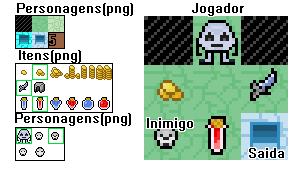
\includegraphics[keepaspectratio=true,scale=0.8]{figuras/fig09-map2.png}
	\caption{Representação do mapa - Objetos utilizados em destaque}
\end{figure}

\subsection{Visibilidade}

É muito comum no gênero \textit{roguelike} o conceito de visibilidade. Um mapa começa escondido e o jogador só pode ver seus itens, inimigos e blocos caso estes estejam em seu campo de visão. 

Existem porém dois tipos de visibilidade. A visibilidade de terreno, ou visibilidade parcial, que identifica o tipo de bloco e itens sobre ele no momento de sua última visualização. Estes blocos costumam ser representados visualmente mais escuros para haver uma diferenciação, e a visibilidade total, onde pode-se ver tudo que está acontecendo naquele espaço. 

A visibilidade é um importante fator de jogabilidade em \textit{roguelikes}, uma vez que muda o modo de pensar e agir de jogadores. Como eles não sabem aonde está a saída, eles devem explorar o mapa às cegas, sem conhecimento do que esta por vir, até que encontrem a saída. 

O sistema simulará jogos utilizando os dois esquemas de visibilidade. Contudo, deve-se ressaltar que não há diversão em explorar um mapa em que já se saiba aonde estão seus inimigos e sua saída, o que constitui um dos principais elementos do gênero.

\subsection{Inimigos e Batalha}

A batalha da simulação ocorre através da tentativa de movimento de uma entidade sobre a outra.
Por ser uma simulação simples e não um jogo complexo, uma batalha decorre-se apenas pela fórmula: 
\begin{equation}
	Dano = atkAtacante - defInimigo
\end{equation}
\begin{equation}
	VidaDefensor = VidaDefensor - Dano
\end{equation}
Eliminando a entidade que chegar a vida zero primeiro. Um jogador sempre terá prioridade de ataque por ser o ator que executa a ação que gera o movimento dos inimigos, sendo a única exceção caso um inimigo seja mais rápido que o jogador e consiga realizar dois ataques em um \textbf{turno}.

Os inimigos terão uma área de observação na qual tomarão a iniciativa de atacar o jogador caso ele adentre esta área. 
A determinação do caminho a ser percorrido pelo inimigo costuma ser direta, devido a pequenas áreas de observações dos inimigos, porém será utilizado o algoritmo $A*$ dado a sua grande eficiência e rapidez em encontrar o melhor caminho possível a um destino. Isto cobrirá casos de mapas com caminhos estreitos e confusos, caso seja necessário. 

\subsubsection{A*}
O algoritmo $A*$ foi escolhido pela sua grande velocidade de processamento tanto de dados grandes ou pequenos e possuir uma implementação relativamente simples. 

Para a implementação no sistema assumiu-se que cada quadrado explorado acarretará em 10 unidades de custo para $H$ e o valor de $G$ seria dado por:
\begin{equation}
	G = (|X_i-X_f| + |Y_i-Y_f|) \times 10
\end{equation}
sendo $_i$ e $_f$ indicações das posições para o nó de origem e destino (final). 

A figura (Figura 10 - \ref{fig10}) demonstra uma iteração do algoritmo. A origem se dá pelo quadrado verde escuro e o fim pelo bloco vermelho. Blocos pretos são obstáculos, enquanto azuis representam nós explorados e verdes descobertos. $F_N$ é o custo de exploração daquele nó. Sempre explorando o nó com a menor soma total. 
\begin{figure}[h]
	\centering
	\label{fig10}
		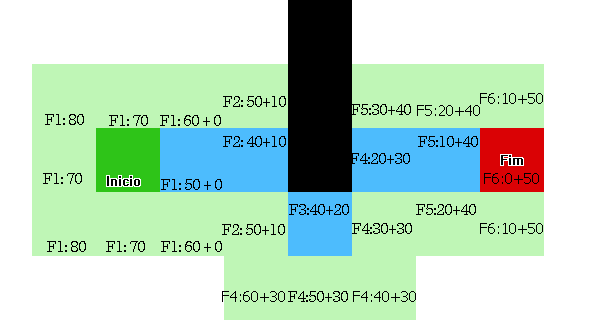
\includegraphics[keepaspectratio=true,scale=0.5]{figuras/fig10-astar.png}
	\caption{Algoritmo A*}
\end{figure}

\subsection{Informações e estados}

A simulação possuirá ainda um sistema de registro (\textit{log}) de mensagens informativas, mostrando danos recebidos e causados para a melhor jogabilidade da simulação por jogadores humanos. 

As mensagens serão mostradas no canto superior da tela e escritas sobre o mapa. Estas informações serão apagadas ao toque de uma tecla ou um movimento realizado pelo jogador. 

Além das mensagens haverá um painel de estados representando os diversos atributos do jogador como seu Ataque, Defesa, Vida e Dinheiro. Este painel possui fim meramente ilustrativo para jogadores humanos possam realizar a simulação sem uma completa desorientação. 


\section{Automatização de jogos}

Para que o sistema se torne uma importante ferramenta para auxiliar no teste da qualidade de mapas, inevitavelmente vários jogos deverão ser realizados sobre um mapa. Trazer jogadores humanos para jogar os mapas e testá-los um a um não traria um dos benefícios esperados do trabalho que é precisamente retirar o usuário do processo inicial de testes e ser capaz de analisar com um certo grau de confiança a qualidade esperada do mapa. 

Desta forma, sente-se a necessidade de que as simulações de jogos do sistema sejam automatizadas. 

\subsection{Robot (BOT)}

Robot, ou BOT em jogos como é mais comumente chamado, é um termo que costuma ser usado para representar a situação na qual um programa ou algoritmo é utilizado para controlar as ações que normalmente seriam efetuadas por jogadores. BOT's devem ser capazes de receber dados do ambiente em que se encontram e processá-los tomando ações de acordo com alguma regra interna estabelecida. O BOT nada mais é do que uma IA capaz de realizar o controle de ações do jogador. 

O sistema utilizará um BOT para simular ações humanas e realizar o jogo de um mapa inúmeras vezes para que ele possa recolher uma grande base de métricas em um pequeno intervalo de tempo, se comparado com o que usuários reais levariam. 

Uma IA porém, mesmo que esteja otimizada, não se compara a um ser humano. Humanos muitas vezes comentem erros ou podem realizar o mesmo jogo de formas diferentes dependendo de seu humor ou personalidade.
Para melhor simular está discrepância entre o processo cognitivo de cada pessoas, o BOT será construído de acordo com parâmetros que o auxiliarão em sua tomada de decisões. 

Desta forma, com apenas alguns ajustes nos parâmetros, pode-se criar uma IA que simularia um usuário com um perfil mais desafiador, ou um usuário com um perfil mais amedrontado. 

\subsubsection{Perfis}

Os principais perfis que pode-se observar em jogadores através de diversos vídeos \cite{letsplay1} \cite{letsplay2} \cite{letsplay3} e análises escritas podem ser divididos em:

\begin{itemize}
	\item \textbf{Explorador} - Aquele jogador que não quer deixar nada para traz, e gosta de explorar o máximo possível do mapa.
	\item \textbf{Ganâncioso} - Aquele jogador que fará tudo para conseguir mais dinheiro ou itens em um mapa. 
	\item \textbf{Corredor} - Aquele jogador que só entra em combate quando extremamente necessário, evitando-os caso possa.
	\item \textbf{Corajoso} - Não deixa nenhum inimigo para tráz, enfrentando todos os inimigos em seu caminho.
	\item \textbf{Esperto} - Um meio termo entro os outros perfis: analisa os riscos e evita batalhas as quais está em desvantagem.
	\item \textbf{Apostador} - Assim como o perfil anterior, analisa a situação, porém aceita riscos caso entenda que exista boas recompensas pelas ações.
\end{itemize}

Cada um destes perfis, apesar de similares, podem afetar completamente a jogabilidade de um mapa. Um nível que talvez seja impossível de se completar ao enfrentar todos os inimigos pode ser extremamente fácil para um perfil \textbf{Corredor} caso os inimigos do mapa sejam lentos e dispersos.

Desta forma, é vital a implementação da inteligência artificial do BOT para que simule as diversas formas de se jogar em um mapa. 

O sistema poderá ainda utilizar um menu para escolher quais perfis deverão ser testados no mapa ou alterar e criar novos perfis pessoais pela alteração dos parâmetros da IA. 

\subsubsection{Algoritmos e parâmetros}

Como dito na seção anterior, é vital a utilização de parâmetros para a conformidade com os diversos tipos de perfis identificados. Aqui será discutido um pouco sobre as técnicas e algoritmos utilizados para movimentação e tomada de decisões do BOT.

Para melhor simular a randomicidade do processamento humano, todos os BOTs utilizados não terão conhecimento qualquer sobre \textit{tiles} que não possam ser visualizados. 

A inteligência artificial do BOT inicia-se na detecção de possíveis alvos e objetos de interesse em sua visão, que são os mesmo para qualquer perfil utilizado.

A IA do BOT é chamada pela ferramenta através do arquivo \textit{playerExplorer.lua}, que estará na pasta \textit{data/scripts}, podendo ser alterado pelos usuários da ferramenta, embora esta não seja uma opção recomendável. 
O \textit{script} será chamado a cada iteração(movimento) do BOT e irá dizer-lher qual a ação deverá ser tomada.

Em seguida é executado um algoritmo similar ao \textit{Depth First Search} \cite{depthsearch}. Este algoritmo inicia-se em um ponto e expande sempre o seu nó descoberto menos distante do caminho até que seja encontrado o destino. O algoritmo utilizado segue mesmo processo de exploração do \textit{Depth First Search} de se explorar sempre os nós mais distantes. Porém o ele é utilizado em formas de iterações, sendo que cada iteração do algoritmo é expandido um nível de movimento e criado um mapa de distâncias. Qualquer objeto de interesse ou bloco não descoberto será considerado como um possível destino (Figura 11 - \ref{fig11}). 

\begin{figure}[h]
	\centering
	\label{fig11}
		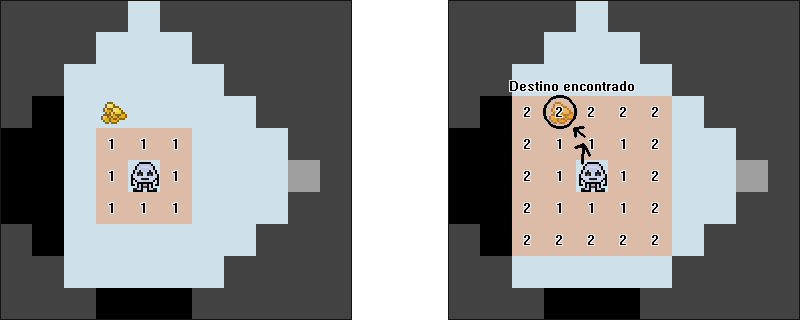
\includegraphics[keepaspectratio=true,scale=0.5]{figuras/fig11-dfs.png}
	\caption{\textit{Depth First Search} em iterações por distancia}
\end{figure}

O \textit{script} então procura por vários possíveis destinos. A cada nó descoberto é feita uma análise para identificar que tipo de bloco e que objetos estão sobre ele, a partir das seguintes regras:
\begin{itemize}
	\item \textbf{Bloco já visto e sem itens ou inimigos} - Nada a fazer
	\item \textbf{Bloco não visto} - Adiciona a lista de \textit{tiles} de interesse.
	\item \textbf{Bloco com itens} - Adiciona a lista de \textit{itens} avistados.
	\item \textbf{Bloco com inimigos} - Adiciona a lista de inimigos avistados.
	\item \textbf{Bloco de terminação do nível} - Adiciona a lista de alvos prioritários. 
\end{itemize}

Vale a pena lembrar que, uma vez que o bloco não seja visível, o BOT não terá conhecimento sobre o que há nele. Podendo até mesmo ser uma parede. 

Este processo continua seqüencialmente junto ao descobrimento de novos blocos. A cada novo nó aberto, o BOT irá realizar a checagem para confirmar se ele chegou ao seu objetivo. 

Para garantir que prioridades de escolha possam ser estabelecidades mais tarde é necessário que sejam avistados mais do que um único destino durante a descoberta, como é o caso dos algortimos de descoberta de caminho. Para se obter tais informações, ao algoritmo avistar o primeiro objeto de interesse, ele irá marcar-se como concluido e executará um número $N$ de iterações adicionais, guardando os novos destinos em uma lista para garantir que existam diversos possíveis alvos e que o BOT possa realizar uma análise mais abrangente. 

Após rodar esta etapa do algoritmo, o \textit{script} possuirá suas devidas listas de \textit{tiles} avistados, itens e inimigos, e iniciará a etapa de processamento destes dados para escolher o seu novo destino (Figura 12 - \ref{fig12}). 

\begin{figure}[h]
	\centering
	\label{fig12}
		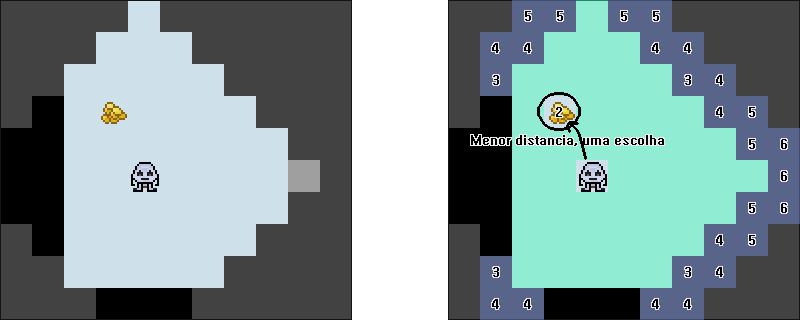
\includegraphics[keepaspectratio=true,scale=0.5]{figuras/fig12-bot.png}
	\caption{Passos simplificados demonstrando o encontro dos blocos pela IA}
\end{figure}

O BOT divide a prioridade de suas escolhas baseado na proximidade, no tipo e nos \textit{parâmetros de ganância} especificados pelo tipo de perfil. 
A IA também tem o conceito de blocos solitários, \textit{singlets}, e tenta priorizar para que não sejam deixados para traz quando não muito custoso (evitando assim movimentos adicionais). Blocos solitários se identificam por um nó do mapa não visto cercado apenas por blocos visíveis. Muitas das vezes este pedaço do mapa será uma área passável, podendo haver itens. Isto dará um custo muito alto de movimento para voltar e re-explorar um bloco esquecido caso seja um perfil explorador ou, num caso extremo, tal bloco pode ser o bloco de saída do mapa. 

A ordem de prioridade de escolha de alvos, sem a alteração de quaisquer \textit{parâmetros de ganância}, são:
\begin{itemize}
	\item 1 - \textit{Singlets} - Blocos solitários
	\item 2 - Itens 
	\item 3 - Inimigos
	\item 4 - Blocos inexplorados
\end{itemize}

O primeiro objeto que entrar na lista de escolhas terá o valor de escolha mínimo igual a sua distância, isto é, todos as outras listas analisadas serão somente adicionadas a lista de possíveis escolhas caso estejam a uma distância mínima menor que o primeiro objeto prioritário encontrado. Porém, para a criação dos diversos perfis é adicionado um \textit{parâmetro de ganância} para adicionar objetos que estejam menos distantes que sua nova distância, dado por:
\begin{equation}
\label{eqn01}
	Dist = dist - greed\Theta
\end{equation}
sendo $Dist$ sua nova distância, $dist$ a distância real do objeto e $greed\Theta$ o parâmetro de ganância do determinado tipo de objeto em questão.

Desta forma é possível alterar a forma com que a IA irá colocar as suas escolhas de acordo com o resultado esperado daquele perfil. Por exemplo, um perfil explorador e ganancioso terá altos parâmetros de ganância para itens e possuirá um maior número de iterações extras para melhor identificar itens nas redondezas, enquanto um perfil Corajoso possuirá altos parâmetros com inimigos (Figura 13 - \ref{fig13}).

\begin{figure}[h]
	\centering
	\label{fig13}
		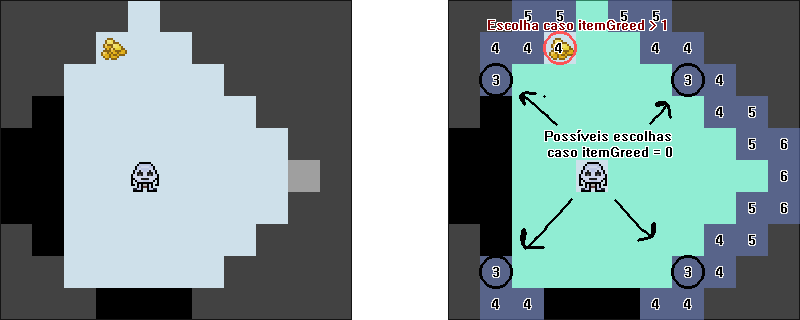
\includegraphics[keepaspectratio=true,scale=0.5]{figuras/fig13-bot2.png}
	\caption{BOT - Alternativas e parâmetros de ganância}
\end{figure}

Ao final do processo, caso não hajam mais meios de filtrar a lista de escolhas restantes, é então escolhido um alvo aleatório dentro das possíveis escolhas.

Por fim, o \textit{script} chamará a função da classe do jogador de dentro do sistema e pedirá que seja construído o caminho até o alvo encontrado. 

Na próxima ação que o BOT for tentar executar, será antes checado se é necessário que haja uma nova análise dos dados para escolha de um novo alvo ou se a IA deverá prosseguir até o seu alvo antes de iniciar o processamento novamente. Isto é testado pela verificação se existe uma rota existente em progresso: caso não haja, simplesmente chama-se a análise novamente.
Porém, caso seja encontrada uma rota, o \textit{script} ainda fará verificações para otimizar a inteligência dele e garantir que não esteja andando para um grupo de inimigos ou um visível beco sem saída, por exemplo.

Desta forma, mesmo havendo rotas presentes para o jogador, caso aviste algum \textbf{novo} inimigo em seu caminho ou realize um movimento de tal forma que o bloco destino esteja visível porém não note a presença de quaisquer novos blocos, irá ser realizada uma nova análise e a escolha de novos destinos (Figura 14 - \ref{fig14}). 
\\\\
\begin{figure}[h]
	\centering
	\label{fig14}
		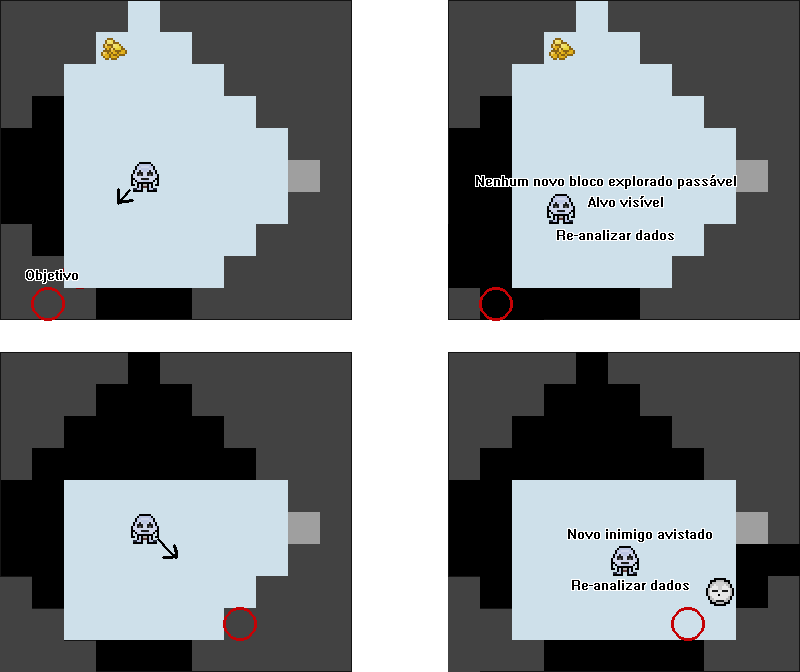
\includegraphics[keepaspectratio=true,scale=0.5]{figuras/fig14-bot3.png}
	\caption{Situações de nova análise dos dados pela IA}
\end{figure}

\section{Métricas}

O sistema terá um módulo de métricas que será capaz de extrair uma série de métricas sobre o decorrer de um jogo simulado. 
As métricas são recolhidas e armazenadas, separando-as para cada mapa e rodada em que foram testadas. 

Desta forma, supondo que existam a métricas $A$, $B$ e $C$ e seja realizado três jogos em um dado mapa.
A ferramenta deverá ser capaz de salvar informações sobre as métricas obtidas $A$, $B$ e $C$ para cada uma daquelas rodadas e exibir também os valores compilados de todas as métricas, disponibilizando para visualização o seu desvio padrão amostral e variância.

O primeiro passo que deve-se fazer é colocar na ferramenta os valores esperados ideais para o mapa de acordo com a expectativa do usuário da ferramenta (provavelmente do \textit{game designer} da equipe). Não há uma qualidade geral de um mapa: um mapa pode ter diferentes objetivos, fica a cargo do usuário decidir que tipo de mapa ele espera. Se é um mapa para um jogo rápido e casual, provavelmente será um mapa com um pequeno tempo de duração e dificuldade. Ou se for um jogo com mais ação, provavelmente seja desejado que haja uma maior quantidade de inimigos e espaço livre para a movimentação.

\subsection{Métricas utilizadas}

As principais métricas identificas durante esta primeira parte do trabalho foram: 

\begin{itemize}
	\item \textbf{Movimentos}:\\
		Indica a quantidade de passos realizados. Através desta métrica é capaz de obter-se a duração de um jogo. O tempo utilizado para a realização de um turno em um jogo do gênero possui uma grande variação, dependendo do momento em que o jogador se encontra, ele pode demorar vários segundos em um único turno em situações de batalha ou vários completar vários turnos em 1 segundo, para corredores e áreas já vistas. A conversão de turnos-segundos utilizada foi 1:1, 1 turno(movimento) igual a 1 segundo. Futuros testes com usuários reais serão necessários para ajustar esta razão de conversão.
	\item \textbf{Itens coletados}:\\
		A métrica indica a quantidade de itens coletados. Isto pode indicar se o nível criado é recompensador o suficiente para o jogador. Esta métrica pode ser tão simples quanto a quantidade de itens coletados, ou a utilização de um fator para representação da importância do item coletado para o jogador. Pode também dividir-se em métrica sobre a quantidade de itens de atributos, que aumentam as habilidades do jogador, ou métrica sobre a quantidade de itens de recuperação. 
	\item \textbf{Dinheiro coletado}:\\
		Indica a quantidade de dinheiro coletado através do jogos. É possível a visualização de quão recompensador foi o jogo, e garantir que os mapas tenham um progresso consistente na evolução do jogo. Por exemplo, para manter um jogador motivado em um jogo é comum que se tenha um progresso constante: grandes variações neste fluxo pode obter efeitos negativos, como a desmotivação do jogador, ou deixar o jogo muito fácil, devido a capacidade de compra de melhores itens muito rápido.
	\item \textbf{Inimigos:}\\
		Esta métrica indica a quantidade de inimigos derrotados. Também pode ser expandida para a quantidade inimigos vistos, porcentagem de inimigos vistos e/ou derrotados. 
		Pode ser utilizada para o balanceamento dos mapas, garantindo que os mapas não possuam uma grande dificuldade. 
	\item \textbf{Vitórias:}\\
		Quantidade de vitórias e derrotas que um BOT obteve em $N$ simulações de partidas em um mapa. Estabelece o quão aceitável o mapa pode ser e a progressão de dificuldade. Jogos casuais, por exemplo, possuem pequeno aumento de dificuldade entre mapas e normalmente costumam ter vitórias fáceis, enquanto jogos \textit{hardcore} costumam ser extremamente difíceis. O jogo \textit{Dungeon Crawl Stone Soup}\footnote{http://crawl.develz.org/wordpress}, voltado ao \textit{roguelike} clássico por exemplo, realizou uma competição \cite{contest} utilizando 1749 pessoas, com uma média de vitórias de 1.37\% e uma média de duração de jogo de 14.8 horas. 
\end{itemize}

\subsection{Análise de métricas}

Uma das grandes partes deste trabalho é descobrir uma forma quantitativa de qualificar de forma significante uma série de dados obtidos dos mapas como bons valores ou ruins de acordo com um intervalo ideal de entrada e através da compilação destes valores identificar se um dado mapa é qualificado como bom ou ruim para aquele tipo de resultados esperados.

Uma das alternativas buscadas para a resolução deste problema foram as hipóteses de teste de comparação, utilizando o teste $t$ de Student.

Uma das primeiras alternativas buscadas para se resolver este problema foi a utilização de distribuições normais de probabilidade e qualificar a porcentagem de chance dos resultados obtidos pertencerem a ela. 

Esta forma de avaliação porém apresenta em sua definição um grande problema para se adequar ao problema. 

Uma distribuição normal de probabilidade estima-se que os valores estejam normalmente distribuídos, isto é, quanto mais próximo a média populacional, maior será a concentração de resultados. Isto não é sempre o que acontece em jogos, a alternativa de explorar primeiro um caminho A ou um caminho B pode mudar significativamente o resultado do jogo, tornando os resultados algo mais próximo a uma série clusterizada, semente em alguns casos obtendo algo próximo ao desvio normal, e mesmo assim contendo também variações anormais.



A análise das métricas será realizada de acordo com parâmetros dispostos pelo usuário da ferramenta. Desta forma, é possível testar se um dado mapa tem a qualidade esperada de um mapa casual ou um mapa mais voltado ao \textit{roguelike} clássico. 

O usuário da ferramenta deverá então ser capaz de inserir no sistema os valores esperados para as métricas ou então escolher ignorá-las por completo, classificando-as como irrelevantes para ele.

A ferramenta será capaz de salvar perfis de métricas para evitar que o usuário tenha que redigitá-las a cada vez que inicie o programa. Poderão ser definidos alguns perfis de métricas padrões escolhidos para acelerar e facilitar o processo para novos usuários.

Através das escolhas das métricas esperadas e métricas obtidas a partir de diversos jogos, a qualidade do mapa será dada por um único fator de qualidade geral, obtida através de uma função de distribuição normal.

O sistema irá gerar uma função de distribuição de densidade \cite{montgomery} para cada uma das métricas a partir dos desvios padrões e valores esperados da agregação dos valores para aquelas métricas. Desta forma, uma dada métrica possui $m$ medidas de acordo com o número de partidas realizadas:
\begin{equation}
data = 
\begin{bmatrix}
	m_1 \\
	m_2 \\
	... \\
	m_n
\end{bmatrix}
\end{equation}

Utilizando estes dados é obtido o valor esperado (média aritmética) e o desvio padrão amostral são obtidos.
\begin{equation}
	\mu = \frac{\sum_{i=1}^{N} m_i}{N}
\end{equation}
\begin{equation}
	\sigma = \sqrt{\sum_{i=1}^{N} \frac{(\mu-m_i)^2}{N(N-1)}}
\end{equation}
sendo $\mu$ o valor esperado (média) e $\sigma$ o desvio padrão. É construído uma função de densidade de probabilidade utilizando o método da distribuição normal. 
\begin{figure}[h]
	\centering
	\label{fig15}
		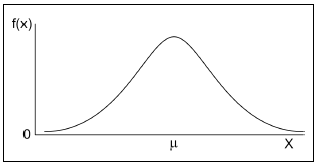
\includegraphics[keepaspectratio=true,scale=0.7]{figuras/fig15-normal.png}
	\caption{Distribuição normal dos dados}
\end{figure}

Por fim, a qualidade para métrica é a probabilidade de que o valor esperado para a métrica, $E(M)$, esteja entre os dados com uma variação $\Delta X$ que será dada por 20\% do valor de $E(M)$.

\begin{figure}[h]
	\centering
	\label{fig16}
		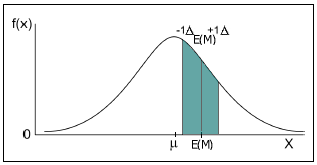
\includegraphics[keepaspectratio=true,scale=0.7]{figuras/fig16-normal2.png}
	\caption{Distribuição normal dos dados}
\end{figure} 

Desta forma, mesmo que uma métrica esperada se aproxime do valor médio, ela mesmo assim não terá uma boa qualidade a menos que os valores tenham pouca variação.

O teste da qualidade utilizando a confiança de 20\% é apenas um teste, na segunda parte do projeto será avaliado a sua relevância quanto sua assertividade e possivelmente deixando a alteração da porcentagem de confiança pelo usuário, caso assim desejar. 

A obtenção na prática dos valores das probabilidades (qualidade) se dá através dos valores $Z$ obtido pelas tabelas das distribuições normais de P(Z < X), conforme apresentado na Equação \ref{eqn02}.
\begin{equation}
\label{eqn02}
	Z = \frac{E(M) - \mu}{\sigma}
\end{equation}
e qualidade  da métrica será então obtida por:
\begin{equation}
\label{eqn03}
	P(Z_1 < Z < Z_2) = P(Z < Z_2) - P(Z < Z_1)
\end{equation}
sendo $Z_1$ e $Z_2$ os limites de aceitação da métrica:
\begin{equation}
\label{eqn04}
	Z_1 = \frac{(E(M) - \Delta X) - \mu}{\sigma}
\end{equation}
\begin{equation}
\label{eqn05}
	Z_2 = \frac{(E(M) + \Delta X) - \mu}{\sigma}
\end{equation}
Por fim, a métrica de qualidade geral do mapa $Q$ será equivalente a média aritmética de todas as qualidades medidas $q_i$. 

\begin{equation}
\label{eqn04}
	Q_{total} = \frac{\sum_{i=1}^{N} q_i}{N}
\end{equation}

\section{Ferramenta auxiliar}

A ferramenta auxiliar foi desenvolvida no \textit{framework} Qt utilizando a linguagem C++ para ajudar no desenvolvimento e observação de mapas, uma vez que construí-los através das regras definidas pelos arquivos \textit{.map} se torna extremamente ineficaz e cansativo se feitos a mão. A ferramenta permite a criação e alteração de mapas, sejam eles feitos a mão ou mapas gerados proceduralmente em tempo de execução.

A interface é adaptável e permite a utilização de janelas flutuantes ou janelas fixadas nas bordas do programa, dando o usuário a liberdade de criar a sua área de trabalho do jeito que lhe seja mais desejável. A interface de edição possui 3 modos de operação para a alteração do mapa que servem para melhor orientar o usuário da ferramenta em relação ao que está sendo feito. 

O primeiro, é o modo de edição de gráficos, neste modo o usuário pode utilizar utilitários como a ferramenta "pincel" para escrita dos blocos no mapa unitáriamente e a ferramenta "retangulo" para a criação de blocos em área. Isto permite a criação mais efetiva do mapa, dando também ao usuário a opção de e selecionar os blocos que desejam ser pintados um a um, ou em grupos. 

O segundo modo é pertinente a edição de entidades, neste modo o usuário poderá criar e alterar entidades para o seu mapa, criar entidades padrões, copiá-las e posicioná-las da forma que desejar. As entidades estão divididas em 3 grandes tipos genéricos: Itens, Inimigos e Dinheiro.


O ultimo modo é o modo de caminhos, com ele é possível visualizar quais blocos são passáveis e quais blocos não serão. Ferramentas para edição rápida como o "retangulo" e a cópia em grupo também se aplicam para esse modo.

Todos os utilitários da aplicação podem ser utilizados através de atalhos de teclado e ela também disponibiliza algumas opções para melhor visualização como a opção de mostrar ou não a malha de quadrados. Por fim, existem 2 botões sinalizando bandeiras que indicam aonde serão as entradas e saídas do mapa, indicando aonde o jogador começará o jogo e aonde poderá chegar para terminá-lo.

Como um outro extra para a ferramenta, foi adotado uma biblioteca \textit{qscintilla} que fornece uma API para a representação de algumas funcionalidades de editores de texto e de código. Com ela foi possível construir uma mini-IDE embutida na ferramenta com a capacidade de interpretar comandos e sintaxes da linguágem \textit{lua} para a criação de \textit{scripts} procedurais e se ter a visualização dos resultados dele na sua frente no mesmo momento, indicando também os erros que ocorreram durante a interpretação dele. 


